The training process was highly demanding concerning the computational resources and the size of the dataset (277,524 images) so it was decided to execute the procedure using cloud resources, specifically in a Kaggle notebook so the dataset can be accessed with ease. In order for the network to be trained properly the arrays X and Y where "fed" to the neurons in batches and for a specific number of times to complete many cycles of training and get more reliable weight values therefore better training results.\\~\\ More specifically the batch size was set to 75 as long as there where available resources to use and reduce the mistakes. The number of training cycles, which are called epochs, was set to 25 because while monitoring the results they where stabilized to certain values. Also, a part of the dataset was used to validate the dataset and continuously adjust the weights to achieve better and more accurate results, by preventing overfitting.\\~\\~\\~\\~\\~\\
Console's output in each epoch : 
\begin{figure}[H]
  \centering
  \subfloat[]{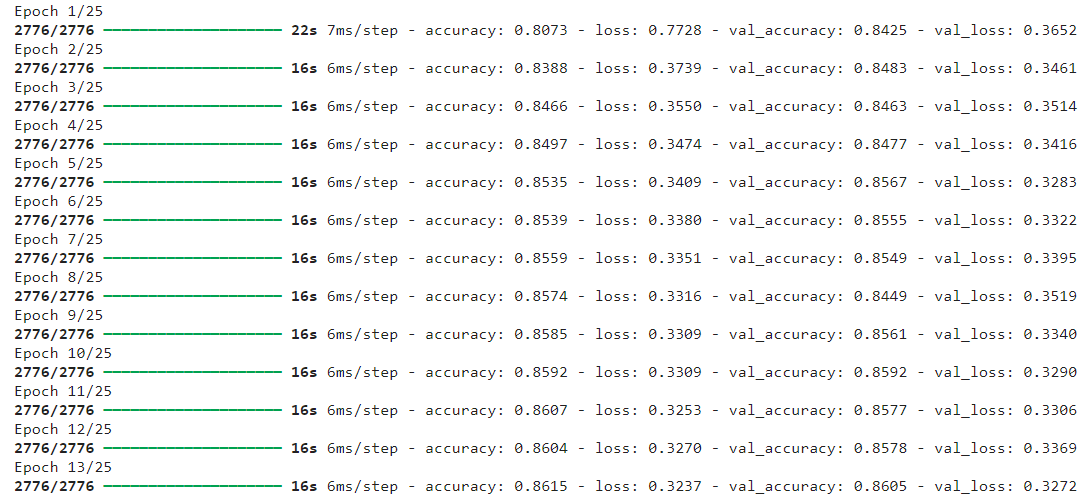
\includegraphics[width=.49\linewidth]{Images/epoch1.png}}\hfill
  \subfloat[] {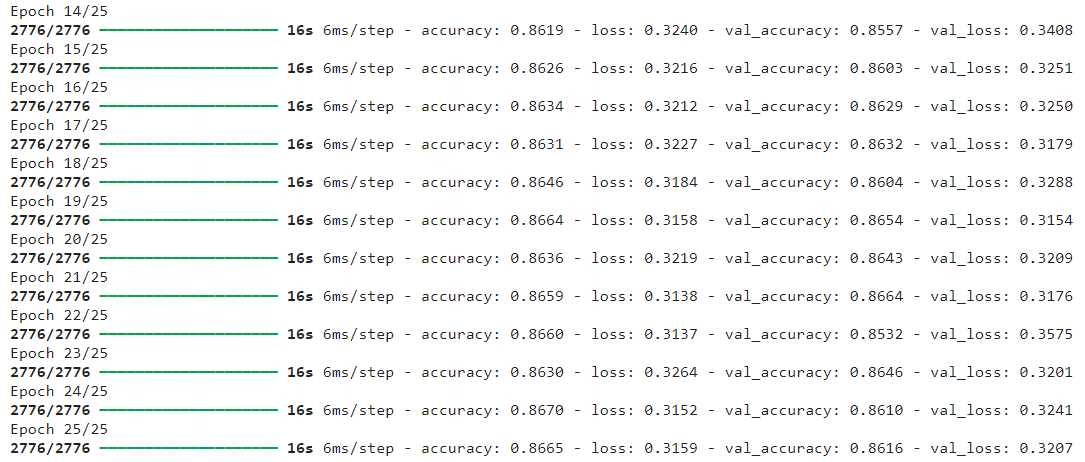
\includegraphics[width=.51\linewidth]{Images/epoch2.png}}
  \caption{Training Process}
\end{figure}
The model's result for it's accuracy and loss in the training process:
\begin{figure}[H]
  \centering
  \subfloat[Accuracy Plot]{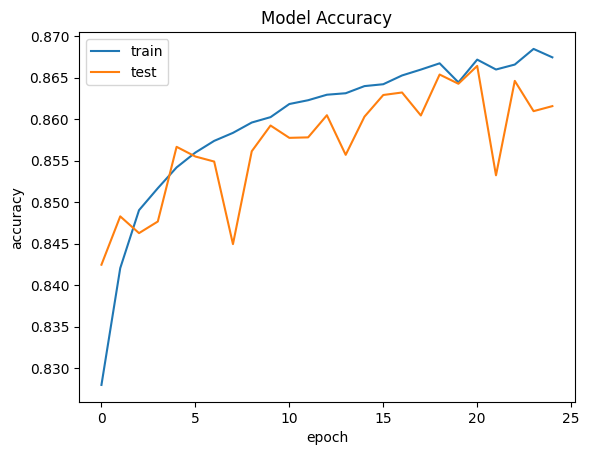
\includegraphics[width=.49\linewidth]{Images/Accuracy.png}}\hfill
  \subfloat[Loss Plot] {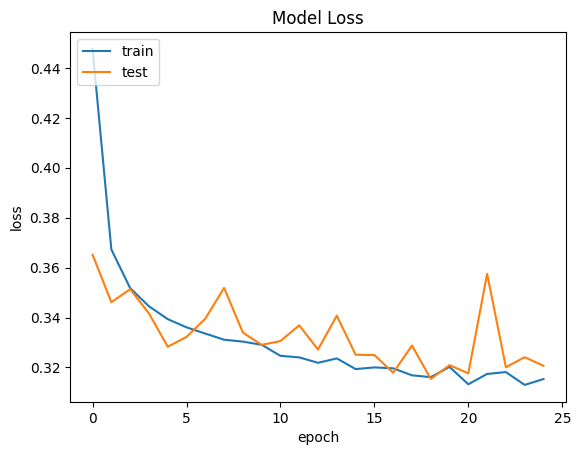
\includegraphics[width=.49\linewidth]{Images/Loss.png}}
  \caption{Training Overview}
\end{figure}

As it seems the average values of the validation and training are pretty close and in a satisfactory level, when taking into account that we deal with image recognition and in order to achieve better results it is needed a more analytic dataset and further training time.